\chapter{Overview of Existing Solutions}
\label{ch:chap2}

\section{Correlation Filter-Based Tracking Methods}
\label{sec:tradi}

% introduce
Correlation Filter (CF)-Based Tracking has emerged as a prominent approach in visual object tracking, known for achieving a good balance between tracking accuracy and speed \cite{feng2019dynamic}. These methods utilize a dynamic model to track the same target across consecutive video frames \cite{du2021overview}. The core idea revolves around learning a correlation filter in the frequency domain to efficiently locate the target in subsequent frames \cite{zhao2020correlation}.

% Step by step
\begin{figure}[h]
    \centering
    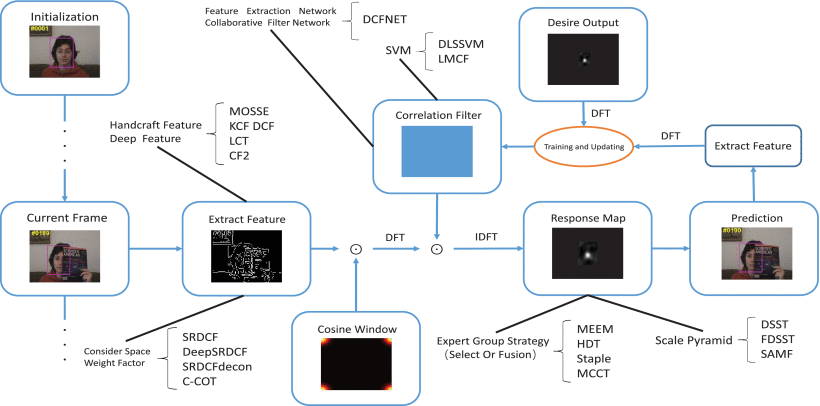
\includegraphics[width=1\linewidth]{images/General framework for correlation-filter-based object tracking.png}
    \caption{General framework for correlation-filter-based object tracking \cite{du2021overview}}
    \label{fig:CF-general-framework}
\end{figure}

The general framework for correlation filter-based object tracking typically involves the following steps \cite{du2021overview}\cite{zhao2020correlation}:
\begin{enumerate}
    \item \textbf{Feature Extraction}: In the initial frame, features are extracted from an image block at the target's location  \cite{du2021overview} \cite{zhao2020correlation}. These features can include handcrafted features like grayscale, Histogram of Oriented Gradients (HOG) \cite{zhao2020correlation}\cite{du2021overview}, and color names (CN) \cite{lin2024motion}, or deep features extracted from Convolutional Neural Networks (CNNs) \cite{du2021overview}\cite{zhao2020correlation}\cite{lin2024motion} . A cosine window is often applied to reduce boundary effects \cite{du2021overview}.

    \item \textbf{Filter Training:} A correlation filter is learned based on the extracted features and a desired output, often a Gaussian-shaped response map centered at the target \cite{feng2019dynamic}\cite{du2021overview} . This learning process aims to create a filter that produces a strong correlation response when convolved with the target and a weak response elsewhere \cite{qiu2024boundary}\cite{du2021overview}. Techniques like the Minimum Output Sum of Squared Error (MOSSE) algorithm represent early and straightforward approaches to filter learning \cite{feng2019dynamic} \cite{du2021overview} \cite{zhao2020correlation}. Kernel Correlation Filters (KCF) further enhance this by utilizing a cyclic matrix to construct training samples and employing kernel functions to handle non-linear features \cite{du2021overview}\cite{zhao2020correlation}\cite{lin2024motion}. Dual Correlation Filters (DCF) represent another early development \cite{du2021overview}.

    \item \textbf{Target Localization:} In subsequent frames, a search window centered around the previous target location is cropped, and features are extracted \cite{zhao2020correlation}. The learned correlation filter is then convolved with these features to generate a response map \cite{du2021overview}\cite{zhao2020correlation}. The location of the maximum response in this map indicates the new position of the target \cite{du2021overview}\cite{zhao2020correlation}. The response map's characteristics, such as its peak value and shape, can also be used for tasks like failure detection \cite{lin2024motion}.

    \item \textbf{Filter Update:} To adapt to changes in the target's appearance and the environment, the correlation filter is typically updated online with new information from the tracked target in the current frame \cite{qiu2024boundary}\cite{du2021overview}\cite{zhao2020correlation}. The learning rate of this update can be adaptively determined based on tracking reliability \cite{du2021overview}.
\end{enumerate}

% Categorization
Correlation filter-based object tracking methods have undergone significant advancements and can be categorized based on several key characteristics \cite{du2021overview}. Early approaches utilized categorized features such as grayscale information, exemplified by the Minimum Output Sum of Squared Error (MOSSE) tracker \cite{feng2019dynamic}\cite{zhao2020correlation}\cite{lin2024motion}. Subsequent developments incorporated more sophisticated handcrafted features like Histogram of Oriented Gradients (HOG) and color names \cite{elmezain2025advancing}\cite{zhang2024webuot}\cite{feng2019dynamic}\cite{lin2024motion}. The integration of deep convolutional neural network (CNN) features has further enhanced performance by providing robust and discriminative representations \cite{feng2019dynamic}\cite{du2021overview}\cite{lin2024motion}. Some trackers leverage a combination of handcrafted and deep features to capitalize on their complementary strengths \cite{zhang2024webuot}\cite{du2021overview}\cite{lin2024motion}.

Another crucial categorization factor is the consideration of the spatial context through space weight factors. Spatially Regularized Discriminative Correlation Filters (SRDCF) were introduced to mitigate boundary effects by penalizing filter coefficients outside the target region \cite{du2021overview}\cite{feng2019dynamic}\cite{lin2024motion}. Variants like DeepSRDCF combine SRDCF with deep features \cite{feng2019dynamic}\cite{du2021overview}, and CSRDCF incorporates channel and spatial reliability \cite{feng2019dynamic}\cite{du2021overview}\cite{zhao2020correlation}. Dynamic Saliency-Aware Regularized CF Tracking (DSAR-CF) refines spatial regularization by integrating object saliency information, allowing the weight map to adapt to shape variations \cite{feng2019dynamic}\cite{du2021overview}\cite{lin2024motion}.
Scale factors represent another important category. Discriminative Scale Space Tracking (DSST) decouples translation and scale estimation to accurately determine the object's size \cite{zhang2024webuot}\cite{feng2019dynamic}\cite{lin2024motion}.

Expert strategies involve utilizing multiple filters or cues and selecting the most reliable one for tracking. Multiexpert Entropy Minimization (MEEM) based on Support Vector Machines (SVM) is an example of this approach \cite{du2021overview}\cite{srigowri2022enhancing}. Methods employing decision-level fusion also fall under this category, combining the outputs of multiple experts based on different features or filter types \cite{lin2024motion}\cite{elmezain2025advancing}. Large Margin Object Tracking with Circulant Feature Maps (LMCF) combines correlation filters with structured SVM for robust tracking \cite{feng2019dynamic}\cite{du2021overview}.

Recent advancements include the development of datasets tailored for specific domains, such as WebUOT-1M for underwater object tracking \cite{zhang2024webuot}. The introduction of Transformer-based architectures in tracking has also shown promising results \cite{zhang2024webuot}. Furthermore, the integration of motion estimation and failure correction modules has been explored to enhance tracking robustness in challenging scenarios, such as in satellite videos \cite{lin2024motion}. The Walsh-Hadamard transform (WHT) has also been investigated for feature extraction in underwater object tracking within a particle filter framework \cite{rout2019walsh}. These categorizations and advancements highlight the continuous efforts to improve the accuracy, robustness, and efficiency of correlation filter-based object tracking algorithms for diverse applications \cite{feng2019dynamic}\cite{du2021overview}\cite{zhao2020correlation}\cite{lin2024motion}.


Correlation filter-based object tracking has evolved significantly with the introduction of various methods that enhance accuracy, robustness, and efficiency. Below is a detailed categorization and description of specific CF-based trackers, highlighting their key features and advancements.

Specific CF-Based Trackers:
\begin{itemize}
    \item MOSSE (Minimum Output Sum of Squared Error) \cite{lin2024motion}: An early, fast tracker using grayscale features.
    
    \item KCF (Kernelized Correlation Filters) \cite{zhao2020correlation}: Utilizes HOG features and kernel functions for improved accuracy and robustness.
    
    \item DCF (Dual Correlation Filters) \cite{feng2019dynamic}: An early approach based on correlation filters.
    
    \item SRDCF (Spatially Regularized Discriminative Correlation Filters) \cite{feng2019dynamic}: Addresses boundary effects using spatial regularization.
    
    \item DeepSRDCF \cite{zhao2020correlation}: Combines deep features with SRDCF
    
    \item C-COT (Continuous Convolution Operators for Tracking) \cite{du2021overview}: Employs continuous convolution operators and deep features, achieving high accuracy.
    
    \item ECO (Efficient Convolution Operators) \cite{feng2019dynamic}: An efficient version of C-COT with a focus on speed and reduced overfitting.
    
    \item DSST (Discriminative Scale Space Tracking) \cite{feng2019dynamic}: Specifically designed for accurate scale estimation.
    
    \item SAMF (Scale Adaptive with Multiple Features) \cite{lin2024motion}: Integrates multiple features and scale estimation.
    
    \item MCCTH (Multicue Correlation Tracker-Based Handcrafted Feature) \cite{du2021overview}: Uses multiple handcrafted feature experts.
    
    \item LMCF (Large Margin With Circulant Feature Maps Tracker) \cite{du2021overview}: Combines correlation filters with structured SVM.
    
    \item DCFNET (Discriminant Correlation Filters Network) \cite{du2021overview}: An end-to-end trainable network for CF tracking.
    
    \item STRCF (Spatial-Temporal Regularized Correlation Filter) \cite{lin2024motion}: Incorporates both temporal and spatial regularization.
    
    \item MACF (Motion-Aware Correlation Filter) \cite{lin2024motion}: Integrates motion estimation for satellite video tracking.
    
    \item CSR-DCF (Discriminative Correlation Filter with Channel and Spatial Reliability) \cite{lin2024motion}: Utilizes channel reliability and spatial confidence.
    
    \item BACF (Background-Aware Correlation Filters) \cite{zhao2020correlation}: Learns from real negative background examples.
    
    \item DSAR-CF (Dynamic Saliency-Aware Regularized CF Tracking) \cite{feng2019dynamic}: Uses dynamic saliency-aware regularization.
\end{itemize}


Correlation filter-based trackers exhibit several notable advantages and limitations. One of the primary strengths of these methods lies in their ability to achieve a favorable balance between tracking accuracy and computational efficiency. This efficiency is largely attributed to the utilization of the Fast Fourier Transform (FFT), which enables rapid convolution operations in the frequency domain \cite{feng2019dynamic}. Additionally, these trackers are capable of learning discriminative filters that effectively distinguish the target from its surroundings \cite{qiu2024boundary}.

However, traditional correlation filter-based trackers also face several challenges. Trackers relying on shallow features are particularly susceptible to environmental factors such as background clutter, occlusions, variations in illumination, and target deformations \cite{feng2019dynamic}\cite{du2021overview}\cite{zhao2020correlation}. Furthermore, the inherent circular shift operation in these methods can lead to undesirable boundary effects, although spatial regularization techniques have been developed to address this issue \cite{feng2019dynamic}. Another limitation is the sensitivity of these trackers to hyperparameter settings, which often require careful tuning to achieve optimal performance \cite{du2021overview}.

While correlation filter trackers offer a balance of efficiency and robustness, ongoing research continues to explore avenues for improvement, including the design of more effective filters, the fusion of complementary features, the development of robust scale estimation and occlusion handling techniques, and the adaptation to specific application scenarios \cite{du2021overview}\cite{zhao2020correlation}. The integration of advanced deep learning architectures and attention mechanisms also represents a promising direction for future work \cite{qiu2024boundary}.


%%%%%%%%%%%%%%%%%%%%
%%%%%%%%%%%%%%%%%%%%
%%% section 2.2 %%%
\section{Deep Learning-Based Tracking Methods}
\label{sec:deep}



Object tracking based on object detection leverages the advancements in object detection algorithms to identify and track objects across video frames. By detecting objects in each frame and associating them over time, these methods provide a robust framework for tracking. Common deep learning-based object detection algorithms can be categorized into two-stage and single-stage algorithms based on convolutional neural networks (CNNs), as well as transformer-based object detection algorithms \cite{zhou2024real}.

\textbf{Two-stage object detection algorithms}, such as Faster R-CNN, operate by first generating region proposals to identify potential object locations. These proposals are then classified and refined to achieve precise object detection and boundary estimation. This method is particularly effective in scenarios requiring high accuracy, as it systematically narrows down the search space for object localization \cite{zhou2024real}.

In contrast, \textbf{single-stage object detection algorithms}, such as YOLO and SSD, predict object classes and locations in a single step. This streamlined process offers a faster and more efficient approach, albeit sometimes at the cost of accuracy. These models, particularly YOLO, have demonstrated reliability in underwater object detection, where computational efficiency is often critical \cite{lotfi2024comparison}.
\begin{figure}[h]
    \centering
    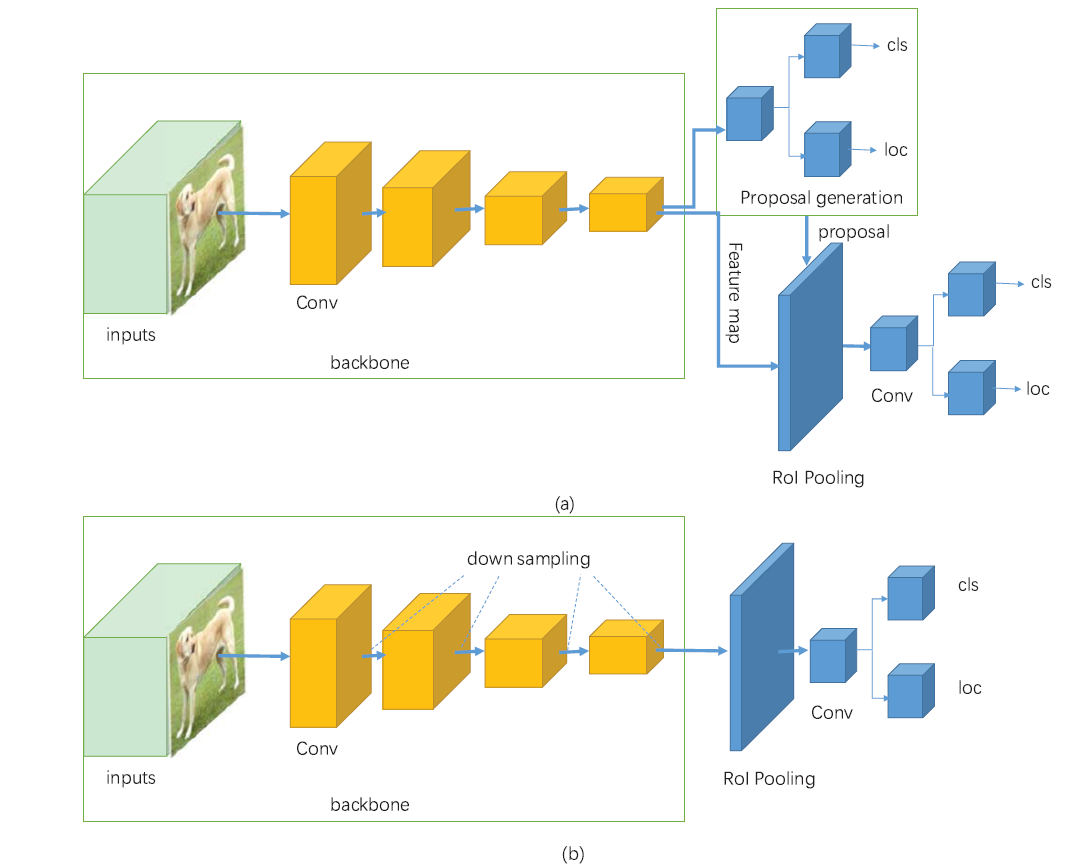
\includegraphics[width=1\linewidth]{images/Object_detector_1stage_vs_2_stage.png}
    \caption{(a) Exhibits the basic architecture of two-stage detectors, which consists of region proposal network to feed region proposals into classifier and regressor. (b) Shows the basic architecture of one-stage detectors, which predicts bounding boxes from input images directly \cite{8825470}.}
    \label{fig:single-two-stage-object-detection}
\end{figure}

Additionally, \textbf{transformer-based object detection algorithms}, such as DETR and RT-DETR, integrate transformers with convolutional neural networks (CNNs) to directly predict object categories and boundaries. This combination enhances efficiency and accuracy, making them a promising choice for modern object tracking applications \cite{zhou2024real}.
\begin{figure}[h]
    \centering
    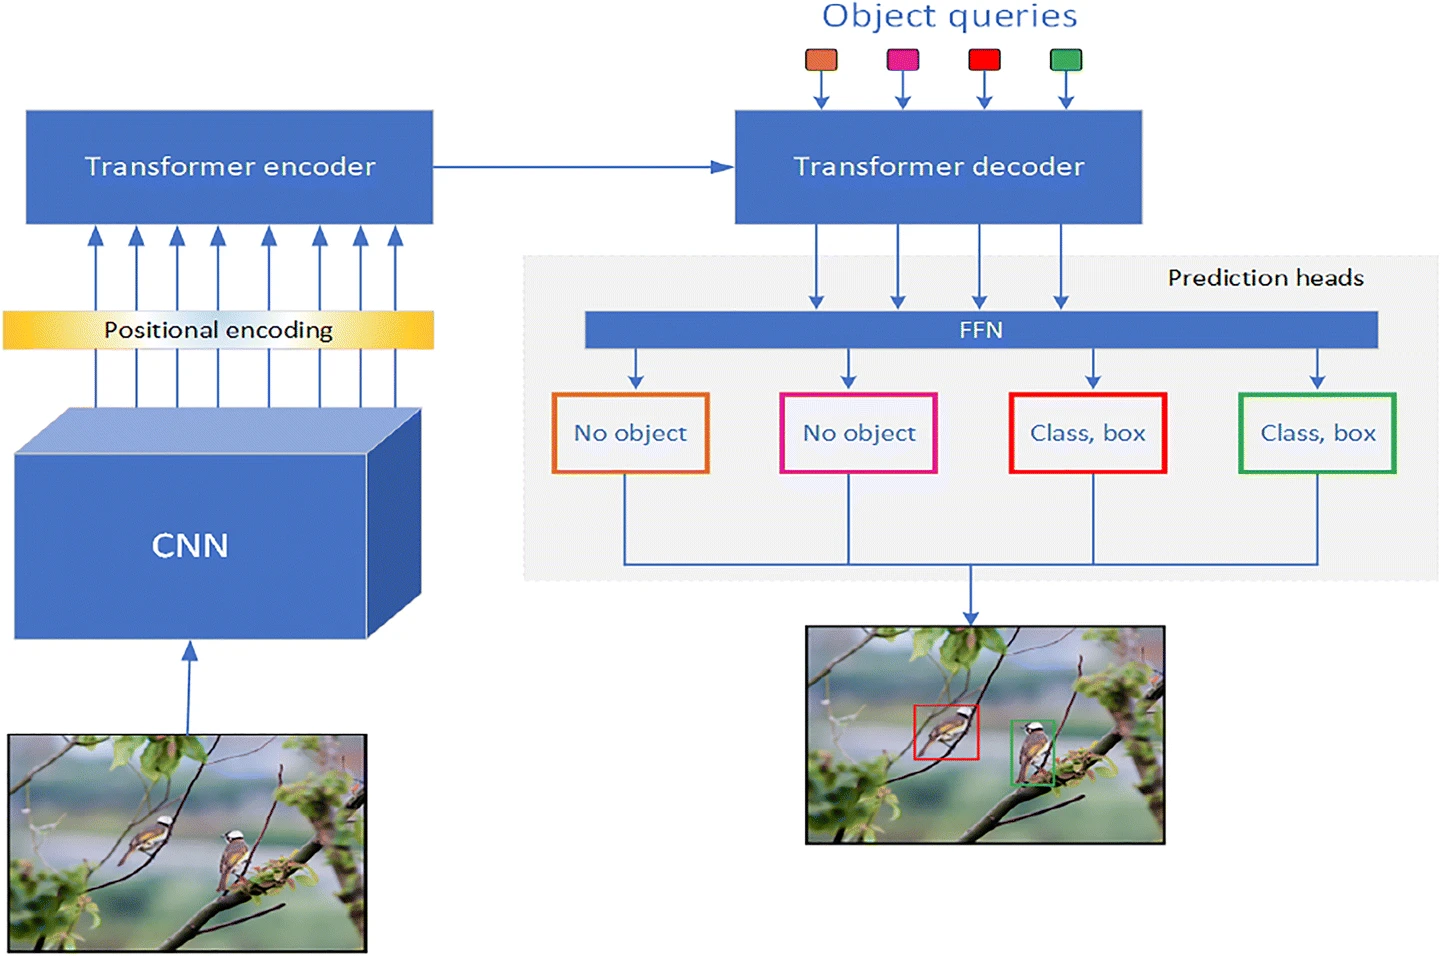
\includegraphics[width=1\linewidth]{images/The process of DETR and its structure.png}
    \caption{The process of DETR and its structure \cite{arkin2023survey}.}
\end{figure}

Despite demonstrating strong performance in terrestrial environments, these algorithms encounter significant challenges in underwater object detection due to factors such as low light conditions and turbid backgrounds \cite{qiu2024boundary}\cite{zhou2024real}\cite{mathias2022occlusion}. Underwater object tracking plays a critical role in applications such as marine resource exploration and military security \cite{qiu2024boundary}. Recent advancements in deep learning have garnered considerable attention for their potential in data-driven underwater image enhancement and object recognition \cite{yang2024lu2net}.

Advanced Deep Learning Techniques Tailored for Underwater Object Tracking (UOT):
\begin{itemize}
    \item \textbf{Knowledge Distillation (KD):} This involves efficiently training a smaller "student" network by learning from a larger, pre-trained "teacher" network. This approach has been applied to UOT, where a teacher model trained on massive open-air data can enhance the tracking performance of a student model dedicated to underwater frames \cite{zhang2024webuot}. Omni-knowledge distillation combines different types of distillation losses, such as token contrastive representation, similarity matrix, feature embeddings, and response maps distillation losses \cite{zhang2024webuot}.
    \item \textbf{Motion-Aware Target Prediction (MATP):} To address model drift caused by similar distractors in underwater environments, a training-free MATP module based on Kalman filtering can be used \cite{zhang2024webuot}. This involves prediction and correction stages to estimate and refine the target's state. UOSTrack also uses motion-based post-processing to mitigate the influence of similar targets \cite{qiu2024boundary}\cite{zhang2024webuot}.
    \item \textbf{Boundary Attention and Sparse Feature Learning:} The DBSF network utilizes a differential boundary attention distribution model to accurately perceive the underwater object edge structure even in noisy and low-resolution images \cite{qiu2024boundary}. It then learns to perceive highly discriminative sparse features on the object structure, reducing the computational demands for edge devices \cite{qiu2024boundary}.
    \item \textbf{Hybrid Training:} Some approaches, like UOSTrack, use hybrid training with both underwater images and open-air sequences to address the sample imbalance problem in underwater datasets \cite{zhang2024webuot}.
    \item \textbf{Siamese network-based trackers}: Siamese networks employ identical neural networks with shared weights to process the target object's initial appearance (template) and subsequent frames (search region) \cite{elmezain2025advancing}. By performing a convolutional feature cross-correlation between these two inputs, Siamese networks learn a similarity function to robustly identify the target across varying conditions and frames \cite{elmezain2025advancing}\cite{zhao2020correlation}\cite{wu2023hybrid}. The tracking task is essentially formulated as a similarity-matching function \cite{wu2023hybrid}.
    \item \textbf{Multi-modal Data:} Leveraging multi-modal data like depth and event information, alongside specialized architectures like multi-scale feature pyramids and transformer-based attention mechanisms, holds significant potential for advancing underwater detection and tracking \cite{elmezain2025advancing}.
\end{itemize}

Deep learning-based object detection models like YOLO, R-CNN, and SSD are used for underwater tracking \cite{lotfi2024comparison}\cite{elmezain2025advancing}. Studies have shown YOLO to be reliable for underwater object detection \cite{lotfi2024comparison}. To enhance temporal stability, YOLO can be merged with SORT \cite{lotfi2024comparison}. Transformer-based architectures are also showing promising results in UOT \cite{mathias2022occlusion}.
\begin{figure}[h]
    \centering
    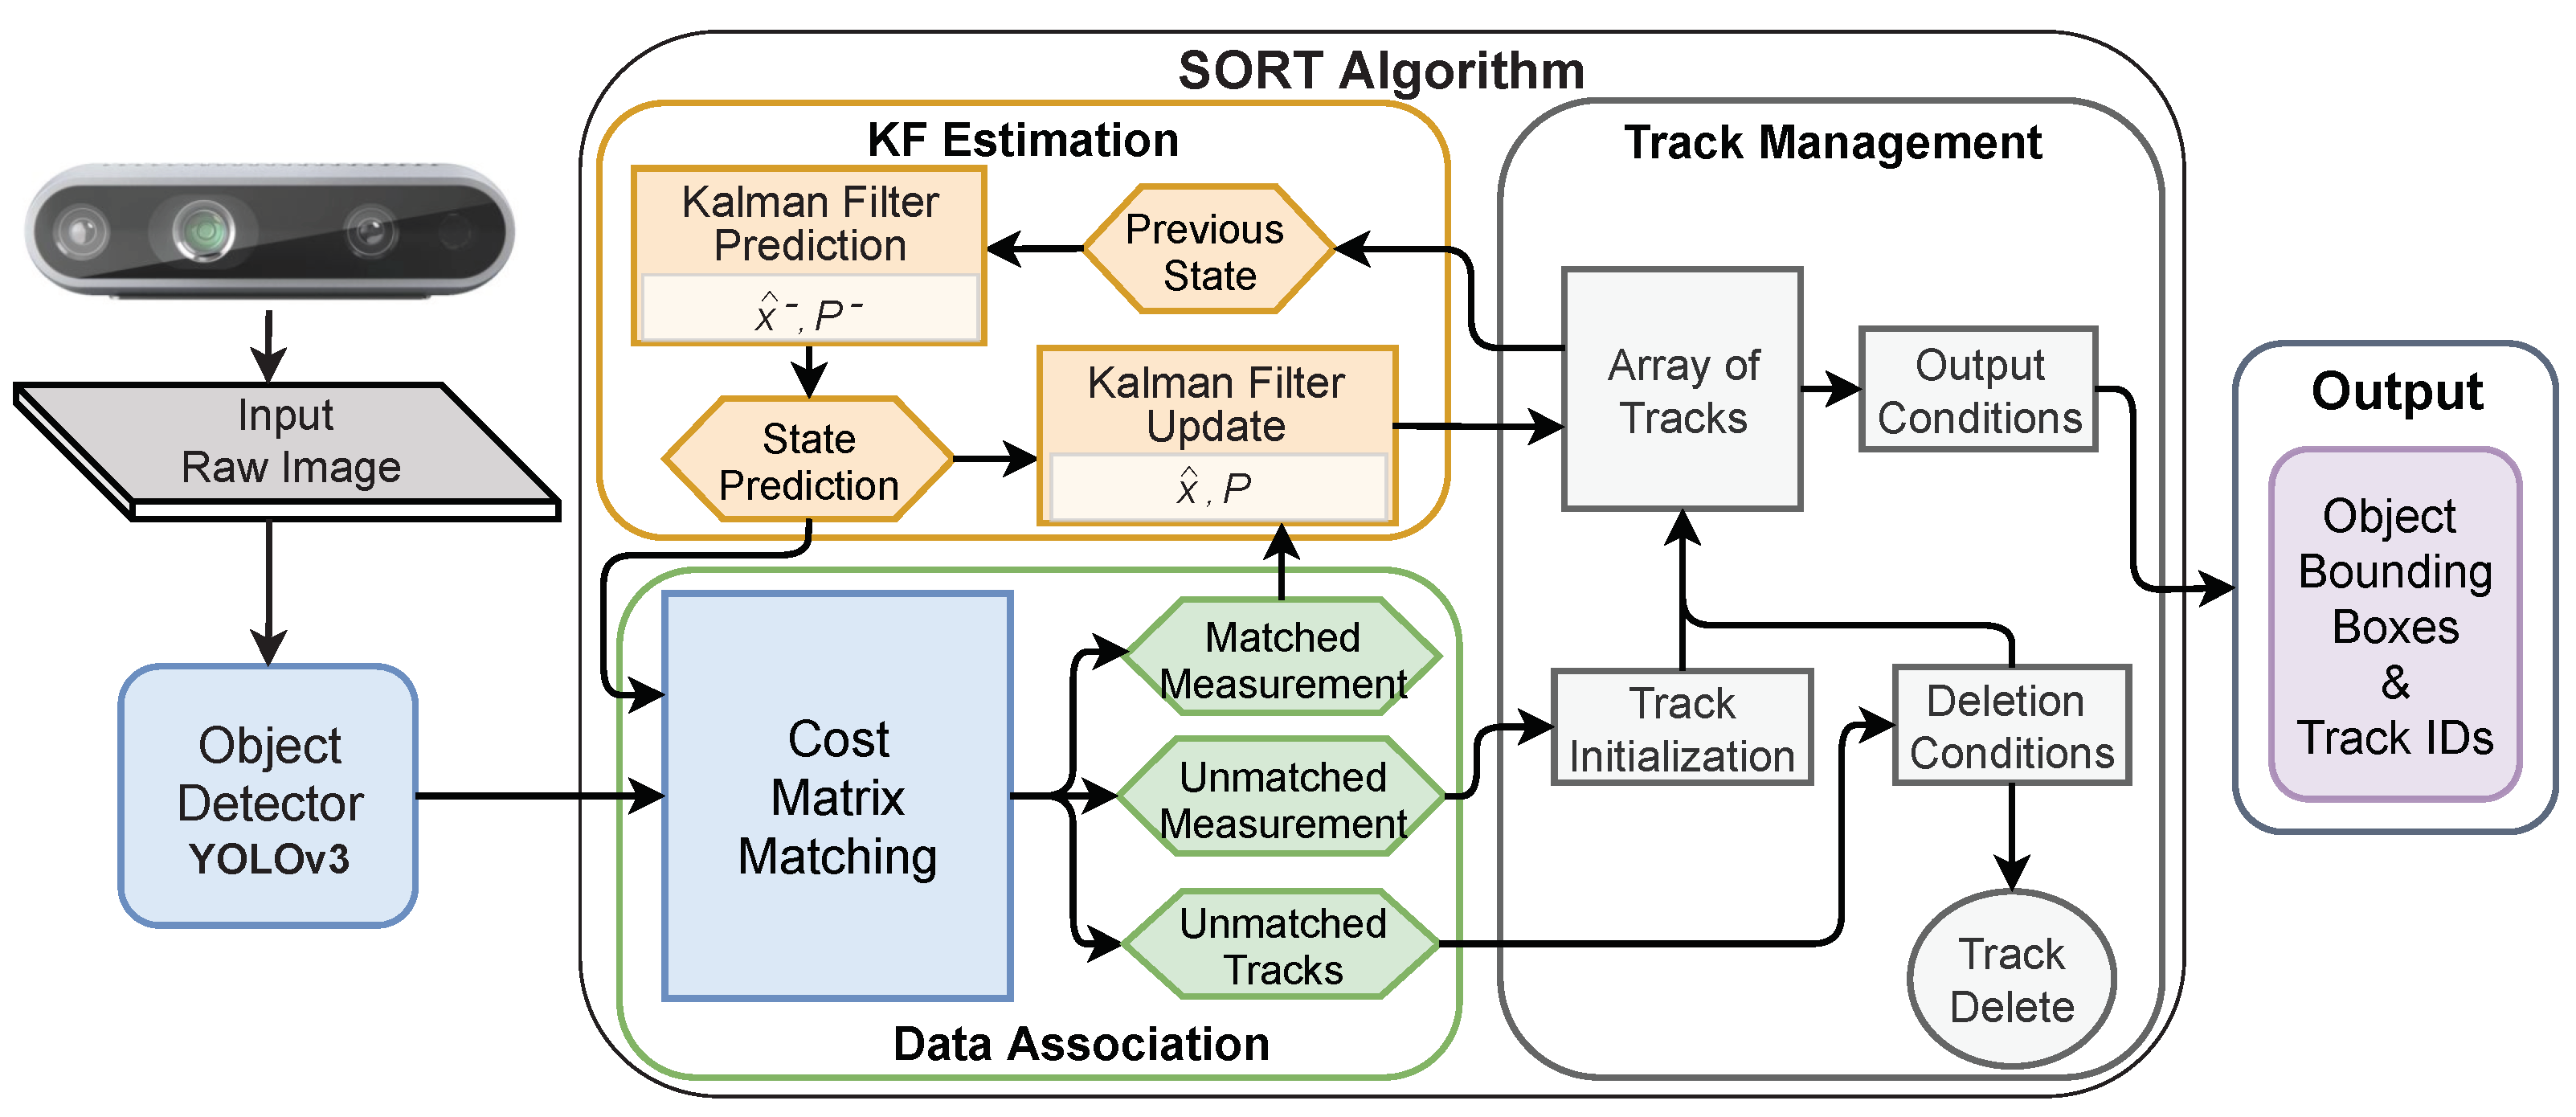
\includegraphics[width=1\linewidth]{images/deepsort.png}
    \caption{Overview of SORT algorithm based YOLOv3 and Kalman filter \cite{pereira2022sort}.}
\end{figure}

% Tracking-by-Detection in Underwater Scenarios:
This paradigm involves using object detection models (like YOLOv3) to detect objects in each frame and then linking these detections across frames using tracking algorithms such as Deep SORT, which can be enhanced with LSTM for handling occlusions, as proposed in the HADSYv3 approach \cite{mathias2022occlusion}\cite{elmezain2025advancing}. This method can be effective in dynamic underwater environments, although its efficacy depends on the quality of the detection algorithm \cite{mathias2022occlusion}.

% dataset and benchmark
Several datasets have been established to promote research in UOT, including UOT32, UOT100, UTB180, VMAT, and UVOT400 \cite{zhang2024webuot}\cite{qiu2024boundary}\cite{rout2019walsh}. However, many lack training sets or have limitations in size and scenario coverage. The WebUOT-1M dataset has been introduced as a larger benchmark to facilitate the development of more powerful deep UOT algorithms \cite{zhang2024webuot}. FishTrack23 is another large-scale dataset specifically for fish tracking \cite{elmezain2025advancing}.

% Performance of Deep Learning Trackers in Underwater Environments:
Evaluations on datasets like WebUOT-1M show that Transformer-based trackers (e.g., OKTrack, UOSTrack, All-in-One, GRM, OSTrack) often perform well \cite{zhang2024webuot}. UOT-specific trackers like OKTrack and UOSTrack, even with plain ViT backbones, can surpass state-of-the-art open-air trackers, highlighting the domain gap between underwater and open-air environments \cite{zhang2024webuot}. Retraining open-air trackers on underwater datasets like WebUOT-1M can effectively reduce this domain gap and improve performance. The DBSF tracker has also demonstrated optimal tracking results on UOT32 and UOT100 benchmarks by focusing on boundary information and sparse confidence features, particularly for edge computing devices \cite{qiu2024boundary}.

% Correlation Filter-Based Tracking Combined with Deep Learning:
Correlation filter (CF) based tracking offers real-time capabilities, and combining it with deep convolutional features has significantly improved performance \cite{qiu2024boundary}\cite{du2021overview}\cite{zhao2020correlation}\cite{lin2024motion}. Algorithms like \textbf{DeepSRDCF}, which uses CNN features, and \textbf{SiamFC}, a fully-convolutional Siamese network, have shown excellent results \cite{zhao2020correlation}. ECO is another efficient correlation filter-based tracker utilizing deep features \cite{zhao2020correlation}\cite{feng2019dynamic}\cite{lin2024motion}. \textbf{MACF} is a motion-aware correlation filter algorithm developed for challenging scenarios like satellite videos with small objects and similar distractors, and it has achieved superior accuracy compared to state-of-the-art trackers \cite{lin2024motion}.

% Challenges and Future Directions in Deep Learning-Based Tracking:
Despite the advancements, challenges remain in UOT, including handling occlusion, small or camouflaged objects, low visibility, optimizing computational efficiency for real-time processing on autonomous systems, and mitigating model drift \cite{qiu2024boundary}\cite{mathias2022occlusion}\cite{zhang2024webuot}\cite{lin2024motion}. Future work includes introducing spatial-temporal features and semi-supervised learning to improve tracking in complex underwater scenes \cite{qiu2024boundary}\cite{mathias2022occlusion}. Enhancing the detection of small or camouflaged objects, optimizing computational efficiency, and improving real-time processing capabilities are also crucial for deployment in autonomous systems \cite{elmezain2025advancing}. For correlation filter-based tracking, future research can focus on designing better filters by considering categorized features, space weight factors, scale factors, and expert strategies, as well as combining manual and deep features \cite{du2021overview}.



%%%%%%%%%%%%%
%%%%%%%%%%%%%
\section{Sensor Fusion-Based Tracking Methods}
Sensor fusion-based approaches in underwater environments leverage data from multiple sensors to enhance surveillance and tracking capabilities \cite{braca2015distributed}\cite{tharmarasa2007large}\cite{uney2022passive}. In contrast to traditional methods that rely on single platforms like submarines or frigates, distributed networks of stationary and mobile sensors, such as autonomous underwater vehicles (AUVs), offer advantages in scalability, robustness, and reliability through intelligent networking \cite{braca2015distributed}. \textbf{Distributed information fusion (DIFFUSION) strategies}, where local information is shared among sensors, are a key aspect of these intelligent networks \cite{braca2015distributed}. This allows for the combination of data from spatially separated sensors to achieve higher performance \cite{braca2015distributed}.

Two primary DIFFUSION schemes are proposed for underwater surveillance: one based on the sharing of local contacts generated by the detection stage, and another based on the sharing of tracks produced by the local tracking stage \cite{braca2015distributed}. In the contact-sharing scheme, contacts are combined at each node using optimal Bayesian tracking based on the random finite set (RFS) formulation \cite{braca2015distributed}. The track-sharing scheme employs a track-to-track (T2T) association and fusion procedure \cite{braca2015distributed}. A local tracker on each AUV provides a set of tracks and their associated covariance matrices, which are then associated and fused with tracks from other AUVs to obtain more accurate state estimates \cite{braca2015distributed}. Unassociated tracks are treated as originating from a single sensor \cite{braca2015distributed}.

The problem of sensor selection within a large network is also critical for optimizing tracking performance under constraints like communication bandwidth \cite{tharmarasa2007large}. Efficient search techniques, such as convex optimization followed by greedy local search, can be employed to determine near-optimal sensor utilization strategies in real-time for multitarget tracking \cite{tharmarasa2007large}. Different approaches to sensor selection include "closest-sensor" strategies, which select sensors nearest to estimated target positions, and more sophisticated methods like "coarse-step" and "fine-step" planning that consider tracking performance over time \cite{tharmarasa2007large}. The posterior Cramér–Rao lower bound (PCRLB) can serve as a basis for network management and as a cost function for optimization \cite{tharmarasa2007large}.

In the context of passive sensor fusion for underwater surveillance, the \textbf{Generalized Labeled Multi-Bernoulli (GLMB)} filter can be used for joint filtering of measurements from multiple sensors, enabling multi-target tracking \cite{uney2022passive}. While detection sets from passive sensors may be staggered in time, the iterated multi-sensor update approach in the GLMB filter has proven sufficiently accurate for simultaneous detections \cite{uney2022passive}. This Bayesian recursion over time allows for long-term integration of sensor data, even when dealing with the non-linearities inherent in bearings-only tracking, often tackled using sequential Monte Carlo methods \cite{uney2022passive}.


\endinput